\documentclass[a4paper,openright,12pt]{report}
\usepackage[spanish]{babel} 
\usepackage{graphicx} 
\usepackage[utf8]{inputenc}
\usepackage{lettrine}
\usepackage{afterpage}
\author{Álvaro Carrasco Carmona}
\title{Trabajo}

\begin{document}

\begin{titlepage}

\begin{center}
\vspace*{-1in}
\begin{figure}[htb]
\begin{center}

\includegraphics[width=8cm]{logo_ugr}
\end{center}
\end{figure}

FACULTAD DE CIENCIAS\\
\vspace*{0.15in}
DEPARTAMENTO DE BIOLOGÍA ORAL \\
\vspace*{0.6in}
\begin{large}
\textbf{AVANCES EN PATOLOGÍA TUMORAL Y NUEVAS
MOLÉCULAS CON APLICACIÓN EN MEDICINA REGENERATIVA} \\
\end{large}
\vspace*{0.2in}
\begin{Large}

\end{Large}
\vspace*{0.3in}
\begin{large}
A work submitted by Álvaro Carrasco for the Regenerative Biomedicine Master \\
\end{large}
\vspace*{0.3in}
\rule{80mm}{0.1mm}\\
\vspace*{0.1in}
\begin{large}
Supervised by: \\
Virginea de Araujo \\
\end{large}
\end{center}

\end{titlepage}
\title{Trabajo de LaTeX}
\maketitle
\twocolumn[
\begin{@twocolumnfalse}
\begin{abstract}

En este trabajo vamos a incluir ejemplos de lo que hemos ido aprendiendo en este curso de LaTeX.

\end{abstract}

\end{@twocolumnfalse}

]

\section*{Introducción}


\lettrine{L}orem ipsum dolor sit amet, consectetur adipiscing elit. Ut dui urna, fermentum eleifend imperdiet quis, dapibus sit amet elit. Aenean volutpat lacus tortor, in pellentesque elit fermentum euismod. Aliquam hendrerit et orci in pretium. Quisque a mauris nec ex ultricies congue ut non est. Nam ultrices sem ut massa ultrices ullamcorper. Suspendisse interdum condimentum odio, non bibendum sem ornare eget. Praesent laoreet euismod est, in sodales tortor aliquet non. Donec est ante, egestas ut nibh vitae, laoreet malesuada sapien. Etiam iaculis facilisis libero eu dapibus. Ut egestas, purus sit amet auctor rutrum, ex arcu interdum velit, id congue nisl ante sed neque. Aliquam erat volutpat. Fusce nec placerat felis. Proin in neque efficitur, hendrerit lectus id, volutpat sem.

Aliquam erat volutpat. Nullam interdum convallis tortor, id tempus orci iaculis at. Orci varius natoque penatibus et magnis dis parturient montes, nascetur ridiculus mus. Suspendisse auctor diam ut tempus euismod. Duis congue ipsum nec eros iaculis scelerisque. Fusce vitae turpis facilisis, consectetur mi luctus, elementum lectus. Pellentesque mattis porttitor ipsum. Quisque posuere mattis suscipit. Morbi vel lacus nisl. Maecenas finibus suscipit arcu, feugiat blandit lectus volutpat nec. Quisque et nulla varius risus accumsan interdum. Ut viverra malesuada arcu. Integer suscipit placerat auctor. Ut in vulputate libero. Vestibulum viverra scelerisque turpis sed finibus. Ut ligula augue, iaculis quis est vel, pellentesque faucibus elit.

Sed vulputate interdum urna, posuere faucibus metus. Lorem ipsum dolor sit amet, consectetur adipiscing elit. Vivamus elementum aliquet nulla vitae scelerisque. Proin porttitor ipsum a dolor bibendum finibus. Sed id vehicula leo, quis elementum lorem. Praesent dictum scelerisque purus, et elementum nibh vehicula sed. Suspendisse rutrum tortor ante, nec convallis dolor tristique in. Donec ullamcorper arcu non sem consequat, eget ultricies massa auctor. Aenean sit amet ultrices lectus. Fusce quis metus semper, vehicula massa in, porta leo. Integer in elit ut libero ultrices sollicitudin. In aliquam molestie eros. Nulla vel mollis leo.


\newpage

\section*{Fórmulas}

\begin{equation}
\phi = \oint_s \vec{E} \cdot d\vec{S} = \frac{q_{enc}}{\varepsilon_0} \quad \textrm {(Ley de Gauss)} 
\end{equation}
\begin{equation}
\oint_S \vec{B} \cdot d\vec{S} = 0 \quad \textrm {(Ley de Gauss para el campo magnético)} 
\end{equation}
\begin{equation}
\oint_C \vec{E} \cdot \vec{dl} = - \frac{d}{dt} \int_s \vec{B} \cdot d\vec{S} \quad \textrm {(Ley de Faraday)} 
\end{equation}
\begin{equation}
\oint_C \vec{B}\cdot d\vec{l} =\mu_0 \int_S \vec{j} \cdot d\vec{S} + \mu_0 \epsilon_0 \frac{d}{dt0} \int_S \vec{E} \cdot d\vec{S} \quad \textrm {(Ley de Ampére)} 
\end{equation}


\begin{figure}[htb]
\begin{center}
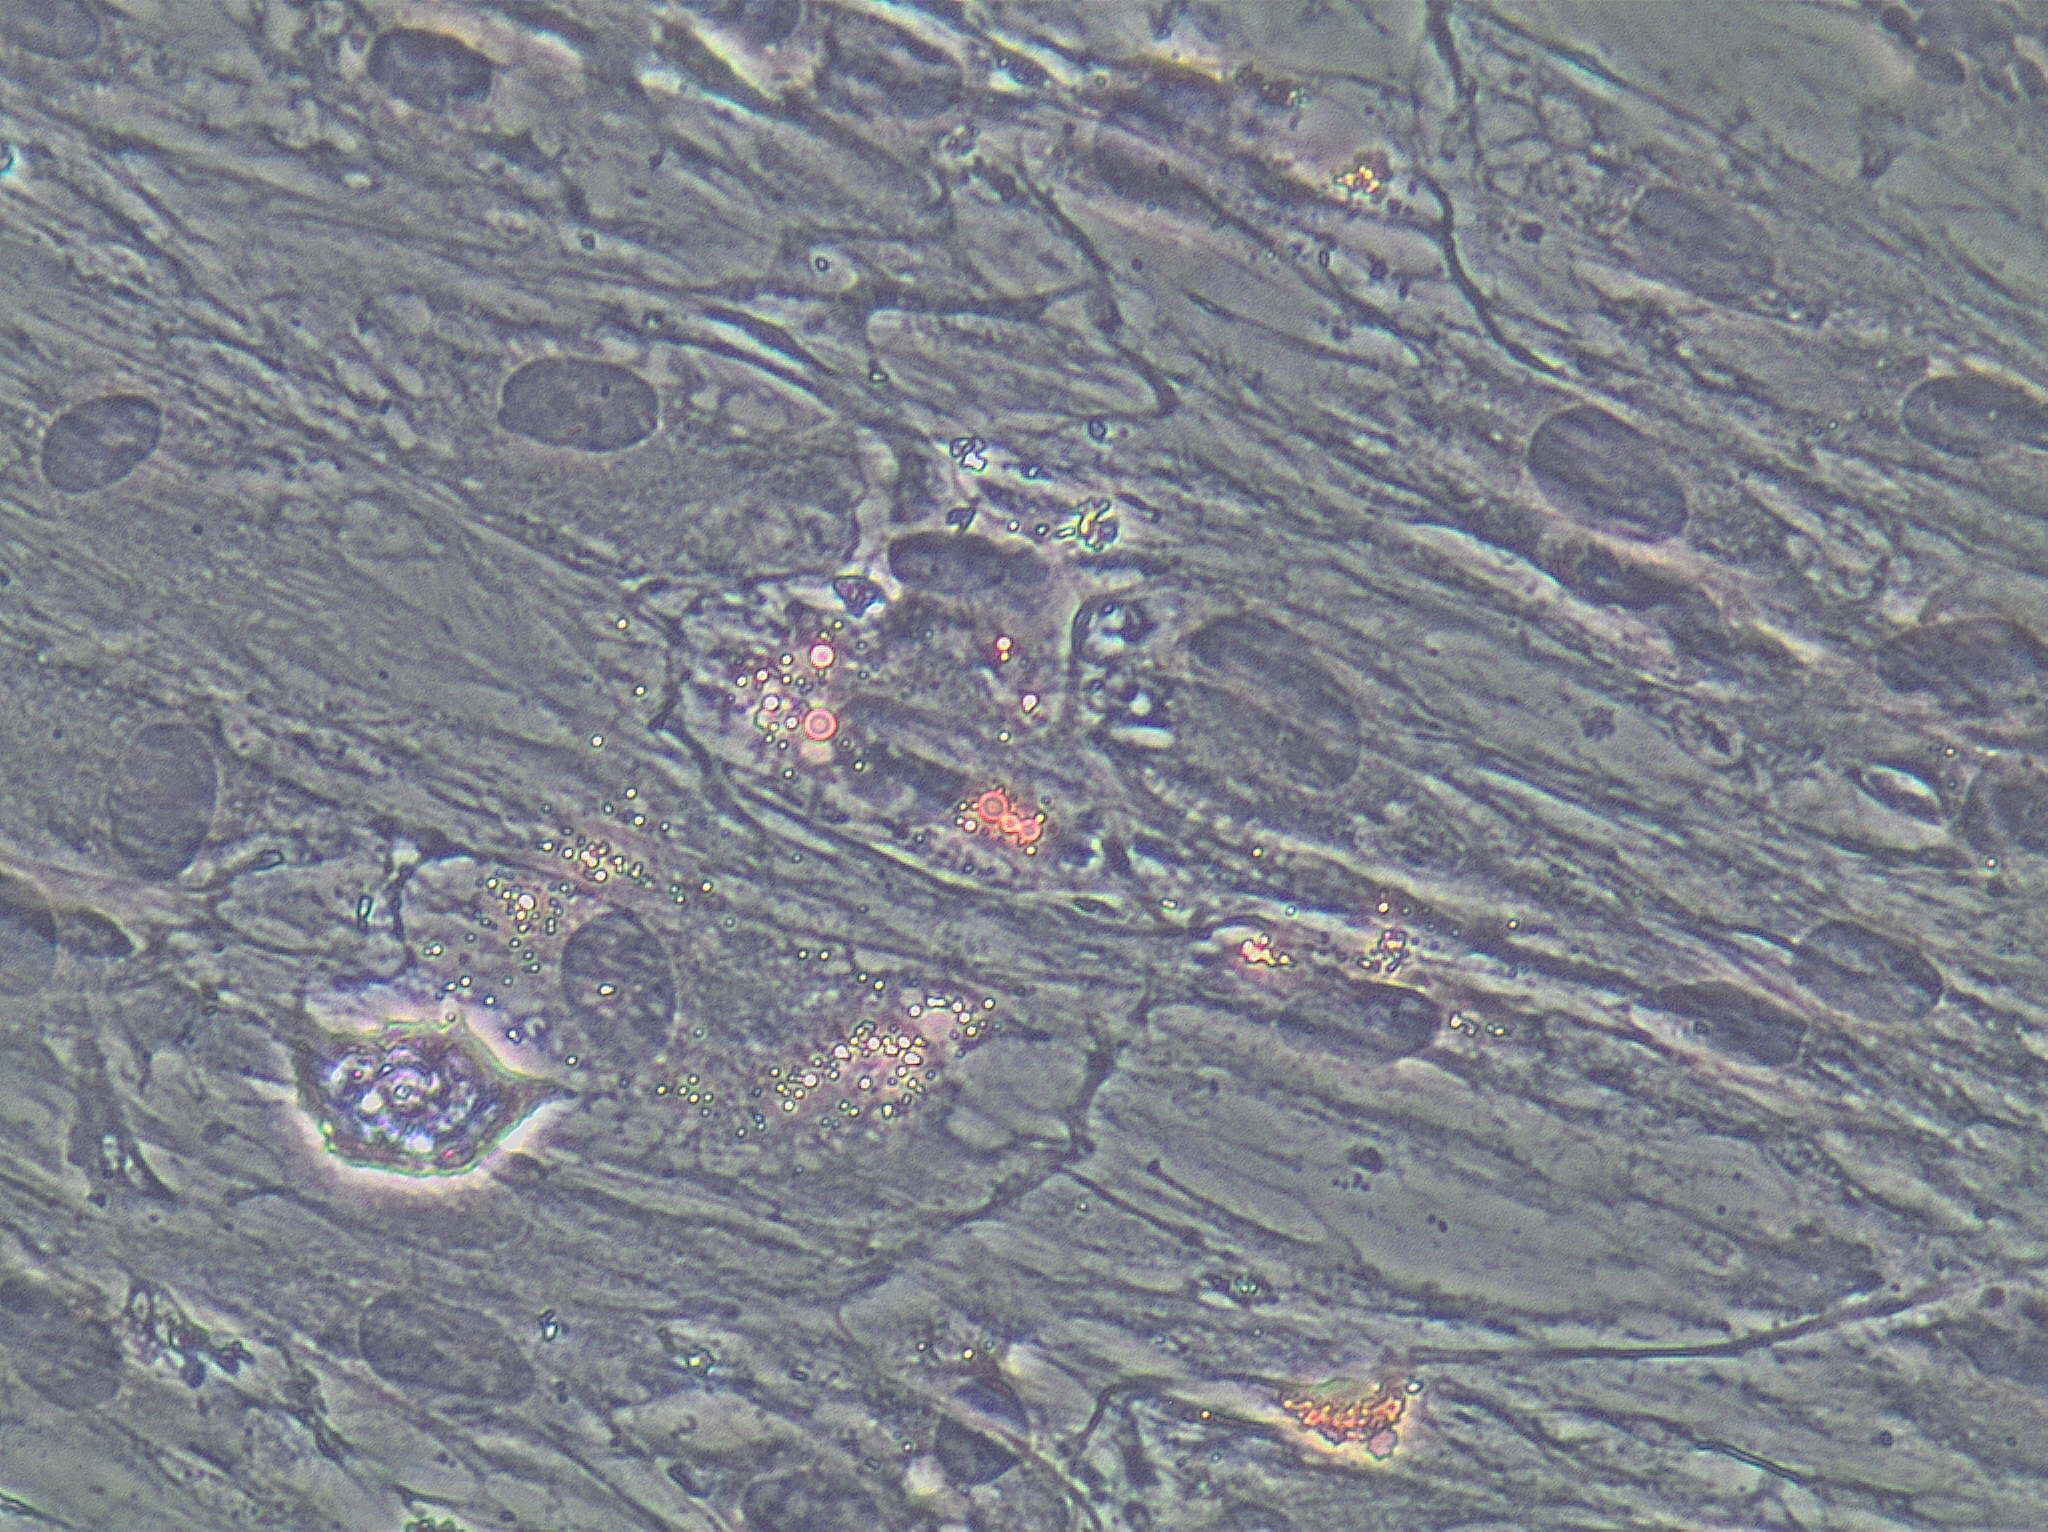
\includegraphics[width=8cm]{Cel1}
\caption{Imagen 1}
\end{center}
\end{figure}

\begin{tabular}{|c|c|}
\hline 
Adipogénico & Osteogénico \\ 
\hline 
DMEM-LG & Neurogénico \\ 
\hline 
\end{tabular} 

\afterpage{\newpage}
\newpage

\twocolumn[
\begin{@twocolumnfalse}

\section*{Referencias}

En esta sección se va a hablar en la bibliografía. En este caso vamos a hablar de los artículos \cite{Livak2001} y \cite{Racz2014}.

\bibliographystyle{unsrt}
\bibliography{Reading_list}


\end{@twocolumnfalse}
]

\afterpage{\null\newpage}

\end{document}